\documentclass[11pt,a4paper]{book}
\usepackage[brazilian]{babel}
\usepackage[utf8]{inputenc}
\usepackage[T1]{fontenc}
\usepackage[inline]{enumitem}
\usepackage{xcolor}
\usepackage{listings}
\usepackage{graphicx}
\usepackage{multicol}
\usepackage{amsmath}
\usepackage{amssymb}

\definecolor{mGreen}{rgb}{0,0.6,0}
\definecolor{mGray}{rgb}{0.5,0.5,0.5}
\definecolor{mPurple}{rgb}{0.58,0,0.82}
\definecolor{backgroundColour}{rgb}{0.95,0.95,0.92}

\lstdefinestyle{CStyle}{
    backgroundcolor=\color{backgroundColour},   
    commentstyle=\color{mGreen},
    keywordstyle=\textbf{\color{black}},
    numberstyle=\tiny\color{mGray},
    stringstyle=\color{mPurple},
    basicstyle=\footnotesize,
    breakatwhitespace=false,         
    breaklines=true,                 
    captionpos=b,                    
    keepspaces=true,                 
    numbers=left,                    
    numbersep=5pt,                  
    showspaces=false,                
    showstringspaces=false,
    showtabs=false,                  
    tabsize=2,
    frame=single,
    escapeinside={(*}{*)},
    language=C
}

\makeatletter
% This command ignores the optional argument for itemize and enumerate lists
\newcommand{\inlineitem}[1][]{%
\ifnum\enit@type=\tw@
    {\descriptionlabel{#1}}
  \hspace{\labelsep}
\else
  \ifnum\enit@type=\z@
       \refstepcounter{\@listctr}\fi
    \quad\@itemlabel\hspace{\labelsep}
\fi}
\makeatother

\newcommand{\onestaritem}{\refstepcounter{enumi}\item[$*$\theenumi.]}
\newcommand{\twostaritem}{\refstepcounter{enumi}\item[$**$\theenumi.]}

\title{Lista 8: Fundamentos Estatísticos para Ciência dos Dados}
\author{Ricardo Pagoto Marinho}

\begin{document}
\maketitle
	\begin{enumerate}
		\item
			\begin{enumerate}[label=\alph*)]
				\item Gerando a matriz \textbf{amostra}:
				\begin{lstlisting}
covMat=matrix(c(4,9,-14,9,30,-44,-14,-44,94),ncol = 3)
L=t(chol(covMat))
mu=c(10,20,-50)
amostra=matrix(0,200,3)
for(i in 1:200){
    z=mvrnorm(1,c(0,0,0),matrix(c(1,0,0,0,1,0,0,0,1),3,3))
    amostra[i,]=mu+L%*%z
}
				\end{lstlisting}
				
				\item Gerando a matriz de covariância $\sum$:
				\begin{lstlisting}
cMat=function(table){
    S=matrix(0,ncol(table),ncol(table))
    mu=apply(table,2,mean)
    for(i in 1:ncol(table)){
        for(j in 1:ncol(table)){
            S[i,j]=sum((table[,i]-mu[i])*(table[,j]-mu[j]))/nrow(table)
        }
    }
	return(S)
}
S=cMat(amostra)

				\end{lstlisting}
				\item Gerando as matrizes de correlação $\rho$ e \textbf{R}:
				
				\begin{lstlisting}
rho=matrix(0,3,3)
for(i in 1:3){
    for(j in 1:3){
        rho[i,j]=cor(amostra[,i],amostra[,j])
    }
}
estCorr=matrix(0,3,3)
for(i in 1:3){
    for(j in 1:3){
        estCorr[i,j]=S[i,j]/sqrt(S[i,i]*S[j,j])
    }
}
				\end{lstlisting}
				
				Coincidentemente, as matrizes de correlação $\rho$ e \textbf{R} ficaram iguais.
			\end{enumerate}
			\item
			
			A função para criar os 5000 valores da matriz R foi implementada da seguinte forma:
			\begin{lstlisting}
function(mu=c(0,0,0),sig=matrix(c(1,0,0,0,1,0,0,0,1),3,3),nlines,ncolums){
    require(MASS)
    L=t(chol(sig))
    amostra=matrix(0,nlines,ncolums)
    R=matrix(0,3,3)
    RR=as.list(numeric(9))
    dim(RR)=c(3,3)
    for(k in 1:5000){
        for(i in 1:nlines){
            z=mvrnorm(1,mu,sig)
            amostra[i,]=mu+L%*%z
        }
        amostra
        S=matrix(0,ncolums,ncolums)
        mu_s=apply(amostra,2,mean)
        for(i in 1:ncolums){
            for(j in 1:ncolums){
                S[i,j]=sum((amostra[,i]-mu[i])*(amostra[,j]-mu[j]))/nlines
            }
        }
        for(i in 1:ncolums){
            for(j in 1:ncolums){
                R[i,j]=S[i,j]/sqrt(S[i,i]*S[j,j])
            }
        }
        for(i in 1:ncolums){
            for(j in 1:ncolums)
                RR[[i,j]][k]=R[i,j]
        }
    }
    return(RR)
}
			\end{lstlisting}
			
			Os histogramas dos 5000 valores de $R_{ij}$, sendo $i\neq j$, já que para $i=j,~R_{ij}=1$, são mostrados na Figura~\ref{fig:fig1}:
			
			\begin{figure}[h]
			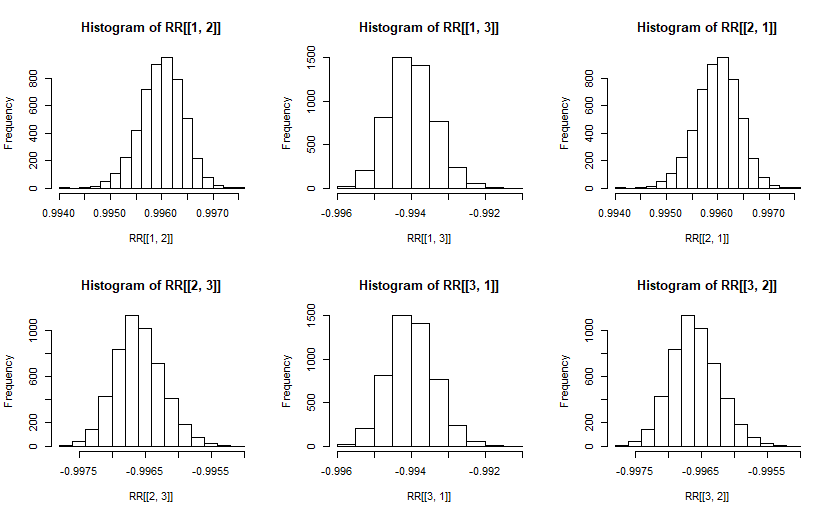
\includegraphics[height=8cm]{Rplot.png}
			\caption{Histograms de $R_{ij}$}
			\label{fig:fig1}
			\end{figure}
			
			Os desvio-padrões aproximados de cada $R_{ij}$ são:
			
			\begin{tabular}{|c|c|}
			\hline
			$R_{ij}$ & Desvio-padrão\\
			\hline
			[1,2] & 0.0015 \\
			\hline
			[1,3] & 0.0005\\
			\hline
			[2,1] & 0.0015\\
			\hline
			[2,3] & 0.0001 \\
			\hline
			[3,1] &0.0005 \\
			\hline
			[3,2] & 0.0001\\
			\hline
			\end{tabular}
			
			\item
				\begin{itemize}
					\item
					Temos que:
					
					\begin{eqnarray*}
						\rho = V^{-\frac{1}{2}}\sum V^{-\frac{1}{2}}
					\end{eqnarray*}
					Sendo que $V^{-\frac{1}{2}}$ é uma matriz quadrada, diagonal com os elementos iguais à $\frac{1}{\sqrt{\sigma_{ii}}}$, onde $\sigma_{ii}$ são os elementos da diagonal principal de $\sum$.
					Portanto,
					\begin{eqnarray*}
						 V^{-\frac{1}{2}}=\left[
						 \begin{tabular}{c c c c}
						 $\frac{1}{\sqrt{3}}$& & & \\
						 &  1 & & \\
						 & &  $\frac{1}{\sqrt{9}}$ & \\
						 & & &  $\frac{1}{\sqrt{4}}$ \\
						 \end{tabular}
						 \right]
					\end{eqnarray*}
					Então:
					\begin{eqnarray*}
					\rho = & \left[
						 \begin{tabular}{c c c c}
						 $\frac{1}{\sqrt{3}}$& & & \\
						 &  1 & & \\
						 & &  $\frac{1}{\sqrt{9}}$ & \\
						 & & &  $\frac{1}{\sqrt{4}}$ \\
						 \end{tabular}
						 \right]\left[
						 \begin{tabular}{c c c c}
						 3 & 0 & 2 & 2\\
						 0 & 1 & 1 & 0\\
						 2 & 1 & 9 & -2\\
						 2 & 0 & -2 & 4\\
						 \end{tabular}
						 \right]
						 \left[
						 \begin{tabular}{c c c c}
						 $\frac{1}{\sqrt{3}}$& & & \\
						 &  1 & & \\
						 & &  $\frac{1}{\sqrt{9}}$ & \\
						 & & &  $\frac{1}{\sqrt{4}}$ \\
						 \end{tabular}
						 \right]
					\end{eqnarray*}
					
					\begin{lstlisting}
s=matrix(c(3,0,2,2,0,1,1,0,2,1,9,-2,2,0,-2,4),ncol=4)
v=matrix(c(1/sqrt(3),0,0,0,0,1,0,0,0,0,1/sqrt(9),0,0,0,0,0.5),ncol = 4)
> m=v%*%(s%*%v)
> m
          [,1]      [,2]       [,3]       [,4]
[1,] 1.0000000 0.0000000  0.3849002  0.5773503
[2,] 0.0000000 1.0000000  0.3333333  0.0000000
[3,] 0.3849002 0.3333333  1.0000000 -0.3333333
[4,] 0.5773503 0.0000000 -0.3333333  1.0000000
					\end{lstlisting}
					\item
					Dado $X'=(X_1,X_2,X_3,X_4)$, um vetor aleatório com vetor esperado $\mathbb{E}(X)=\mu=(0,1,0,-1)'$ e matriz de covariância
					
					\begin{eqnarray*}
						\sum=\left[
						\begin{tabular}{c c c c }
						 3 & 0 & 2 & 2\\
						 0 & 1 & 1 & 0\\
						 2 & 1 & 9 & -2\\
						 2 & 0 & -2 & 4\\
						\end{tabular}
						\right]
					\end{eqnarray*}
					
					Particionando
					\begin{eqnarray*}
					X=\left[
					\begin{tabular}{c}
					$X_1$\\
					$X_2$\\
					\hline
					$X_3$\\
					$x_4$\\
					\end{tabular}
					\right]=
					\left[\begin{tabular}{c}
					$X^{(1)}$\\
					\hline
					$X^{(2)}$\\
					\end{tabular}
					\right]
					\end{eqnarray*}
					
					Sabe-se que ($X^{(1)},X^{(2)}$) é uma normal bivariada e combinação linear de $X'=(X_1,X_2,X_3,X_4)$.
					
					\begin{eqnarray*}
						\mathbb{E}(X^{(1)})=\left(
						\begin{tabular}{c}
						0\\
						1\\
						\end{tabular}
						\right)
					\end{eqnarray*}
					\item
					Como $X^{(1)}$ é combinação linear de $X_1$ e $X_2$, logo:
					
					\begin{eqnarray*}
						\mathbb{E}(AX^{(1)})=(1,-1)\left(
						\begin{tabular}{c}
						0\\
						1\\
						\end{tabular}
						\right)
					\end{eqnarray*}
					\begin{lstlisting}
A=c(1,-1)
> m12=matrix(c(0,1),ncol=1)
> e=A%*%m12
> e
     [,1]
[1,]   -1
					\end{lstlisting}
					
					Portanto, $\mathbb{E}(AX^{(1)})=-1$
					
					\item
					A matriz de covariância $\sum$ de $X^{(1)}$ é
					
					\begin{eqnarray*}
						\sum = \left[
						\begin{tabular}{c c}
						3 & 0\\
						0 & 1\\
						\end{tabular}
						\right]
					\end{eqnarray*}
					
					\item
					$Cov(AX^{(1)})=(1,-1)Cov(X^{(1)})\left(
					\begin{tabular}{c}
					1\\
					-1\\
					\end{tabular}
					\right)$
					
					Logo:
					\begin{lstlisting}
A=c(1,-1)
cov12=matrix(c(3,0,0,1),ncol=2)
> A%*%(cov12%*%t(t(A)))
     [,1]
[1,]    4
> 
					\end{lstlisting}
					
					\item
					\begin{eqnarray*}
						\mathbb{E}(X^{(2)})=\left(
						\begin{tabular}{c}
						0\\
						-1\\
						\end{tabular}
						\right)
					\end{eqnarray*}
					
					\item
					Temos que:
					
					$\mathbb{E}(BX^{(2)})=B\mathbb{E}(X^{(2)})$
					
					\begin{lstlisting}
mu34=matrix(c(0,-1),ncol = 1)
> B=matrix(c(1,1,-1,2),ncol = 2)
> B%*%mu34
     [,1]
[1,]    1
[2,]   -2
					\end{lstlisting}
					\item
					$Cov(AX^{(2)})=\left[
					\begin{tabular}{c c}
					9 & -2\\
					-2 & 4\\
					\end{tabular}
					\right]
					]$
					
					\item
					\begin{eqnarray*}
						Cov(BX^{(2)})=&BCov(X^{(2)})B'
						=&\left[
						\begin{tabular}{c c}
						1 & -1\\
						1 & 2\\
						\end{tabular}
						\right]
						\left[
						\begin{tabular}{c c}
						9 & -2\\
						-2 & 4\\
						\end{tabular}
						\right]
						\left[
						\begin{tabular}{c c}
						1 & 1\\
						-1 & 2\\
						\end{tabular}
						\right]
					\end{eqnarray*}
					
					\begin{lstlisting}
cov2=matrix(c(9,-2,-2,4),ncol = 2)
> B%*%(cov2%*%t(B))
     [,1] [,2]
[1,]   17   -1
[2,]   -1   17
					\end{lstlisting}
				\end{itemize}
			\item
			Como X é combinação linear de $Y_1$,
			\begin{eqnarray*}
			\mathbb{E}(Y_1)=\mathbb{E}(c'_1X)=c'\mu
			\end{eqnarray*}
			onde $c'_1=(\frac{1}{4},-\frac{1}{4},\frac{1}{2})$ e $\mu=(-1,0,2)$, portanto,
			
			\begin{eqnarray*}
			\mathbb{E}(Y_1)=\mathbb{E}(c'_1X)=c'\mu = -\frac{1}{4}+0+1=\frac{3}{4}
			\end{eqnarray*}
			
			Além disso, a variância $\mathbb{V}(Y_1)=c'_1\sum c_1$, onde
			
			\begin{eqnarray*}
			\sum=\left[
			\begin{tabular}{c c c}
			1 & 2 & -2\\
			-2 & 5 & 0\\
			0 & 0 & 2\\
			\end{tabular}
			\right]
			\end{eqnarray*}
			
			Logo,
			\begin{lstlisting}
c1=c(1/4,-1/4,1/2)
> sig=matrix(c(1,-2,0,-2,5,0,0,0,2),ncol = 3)
> c1%*%(sig%*%t(t(c1)))
      [,1]
[1,] 1.125
			\end{lstlisting}
			
			Para $Y_2$ fazemos a mesma coisa utilizando o vetor 'c' correto, ou seja: $c'_2=(\frac{1}{4},\frac{1}{4},-\frac{1}{2})$.
			Portanto,
			\begin{eqnarray*}
				\mathbb{E}(Y_2)=\mathbb{E}(c'_2X)=c'\mu = \frac{1}{4}+0-1=-\frac{5}{4}
			\end{eqnarray*}			
			e a variância $\mathbb{V}(Y_2)=c'_2\sum c_2$:
			\begin{lstlisting}
c2=c(1/4,1/4,-1/2)
> c2%*%(sig%*%t(t(c2)))
      [,1]
[1,] 0.625
			\end{lstlisting}
			
			Para obter a distribuição conjunta de $(Y_1,Y_2)$ precisamos da esperança $\mu_{12}$ e da matriz de covariância$\sum_{12}$.
			$\mu_{12}$ é obtido a partir das esperanças de $Y_1$ e $Y_2$, ou seja, $[\frac{3}{4},-\frac{5}{4}]$.
			Os elementos (1,1) e (2,2) da matriz de covariância são conhecidos e foram calculados anteriormente, \textit{i.e.}, $\sigma_{11}=1.125$ e $\sigma_{22}=0.625$.
			Os elementos (1,2) e (2,1) são o mesmo, já que a matriz é simétrica e são encontrados nos elementos (1,2),(2,1) da matriz:
			\begin{eqnarray*}
				\left[
				\begin{tabular}{c}
				$c_1$\\
				$c_2$\\
				\end{tabular}
				\right]
				\sum \left[c_1,c_2
				\right]
			\end{eqnarray*}
			\begin{lstlisting}
> c=cbind(c1,c2)
> t(c)%*%(sig%*%c)
       c1     c2
c1  1.125 -0.750
c2 -0.750  0.625
			\end{lstlisting}
			Logo, $\sigma_{12}=\sigma_{21}=-0.75$.
			Portanto:
			
			\begin{eqnarray*}
			\left(
			\begin{tabular}{c}
			$Y_1$\\
			$Y_2$\\
			\end{tabular}
			\right)\sim N_2
			\left(
			\left[
			\begin{tabular}{c c}
			$\frac{3}{4}$\\
			$-\frac{5}{4}$\\
			\end{tabular}
			\right],
			\left[
			\begin{tabular}{c c}
			 1.125 & -0.750\\
			-0.750  & 0.625\\
			\end{tabular}
			\right]
			\right)
			\end{eqnarray*}	
			
			\item
			Para saber se duas v.a.s $i$ e $j$ são independentes, basta olhar para os elementos $i,j$ da matriz de covariância.
			Caso sejam 0, elas serão independentes, se for diferente de 0, elas não são.
			No caso de sub-vetores de variáveis, tem que olhar para a sub-matriz $i,j$ na matriz de covariância particionada.
			Portanto:
			\begin{itemize}
			\item Não são independentes
			\item São independentes
			\item São independentes
			\item São independentes
			\item São independentes pois
			\begin{eqnarray*}
			Cov(X_2,X_2+\frac{5X_1}{2}-X_3) = Cov(X_2,X_2)+\frac{5}{2}Cov(X_2,X_1)-Cov(X_2,X_3) =\\ 5+\frac{5}{2}-2-0 = 0
			\end{eqnarray*}
			\end{itemize}
		\item
		\begin{lstlisting}
stif= matrix(scan("stiffness.txt"), ncol=5, byrow=T)
x = stiffness[,1:4]
mu = apply(x, 2, mean)
sigm = cov(x)
dev = x - matrix(mu, nrow=nrow(x), ncol=ncol(x), byrow=T)
d2est = diag(desv %*% (solve(sig) %*% t(dev)))
d2 = mahalanobis(x, mu, sig)
plot(d2, d2est)
anomal = d2 > qchisq(0.95,4)
x[anomal,]
nanom = sum(anomal)
pairs(rbind(x, x[anomal,]), pch="*", col=rep(c("black", "red"), c(nrow(x), nanom)))
		\end{lstlisting}
		\item
		\begin{itemize}
		\item
		Setosa:
		\begin{lstlisting}
apply(iris[iris$Species=="setosa",1:4],2,mean)
Sepal.Length  Sepal.Width Petal.Length  Petal.Width 
       5.006        3.428        1.462        0.246 
> round(cov(iris[iris$Species=="setosa",1:4]),3)
             Sepal.Length Sepal.Width Petal.Length Petal.Width
Sepal.Length        0.124       0.099        0.016       0.010
Sepal.Width         0.099       0.144        0.012       0.009
Petal.Length        0.016       0.012        0.030       0.006
Petal.Width         0.010       0.009        0.006       0.011
round(cor(iris[iris$Species=="setosa",1:4]),3)
             Sepal.Length Sepal.Width Petal.Length Petal.Width
Sepal.Length        1.000       0.743        0.267       0.278
Sepal.Width         0.743       1.000        0.178       0.233
Petal.Length        0.267       0.178        1.000       0.332
Petal.Width         0.278       0.233        0.332       1.000
		\end{lstlisting}
		
		Versicolor:
		\begin{lstlisting}
apply(iris[iris$Species=="versicolor",1:4],2,mean)
Sepal.Length  Sepal.Width Petal.Length  Petal.Width 
       5.936        2.770        4.260        1.326 
> round(cov(iris[iris$Species=="versicolor",1:4]),3)
             Sepal.Length Sepal.Width Petal.Length Petal.Width
Sepal.Length        0.266       0.085        0.183       0.056
Sepal.Width         0.085       0.098        0.083       0.041
Petal.Length        0.183       0.083        0.221       0.073
Petal.Width         0.056       0.041        0.073       0.039
> round(cor(iris[iris$Species=="versicolor",1:4]),3)
             Sepal.Length Sepal.Width Petal.Length Petal.Width
Sepal.Length        1.000       0.526        0.754       0.546
Sepal.Width         0.526       1.000        0.561       0.664
Petal.Length        0.754       0.561        1.000       0.787
Petal.Width         0.546       0.664        0.787       1.000
		\end{lstlisting}
		
		Virginica:
		\begin{lstlisting}
apply(iris[iris$Species=="virginica",1:4],2,mean)
Sepal.Length  Sepal.Width Petal.Length  Petal.Width 
       6.588        2.974        5.552        2.026 
> round(cov(iris[iris$Species=="virginica",1:4]),3)
             Sepal.Length Sepal.Width Petal.Length Petal.Width
Sepal.Length        0.404       0.094        0.303       0.049
Sepal.Width         0.094       0.104        0.071       0.048
Petal.Length        0.303       0.071        0.305       0.049
Petal.Width         0.049       0.048        0.049       0.075
> round(cor(iris[iris$Species=="virginica",1:4]),3)
             Sepal.Length Sepal.Width Petal.Length Petal.Width
Sepal.Length        1.000       0.457        0.864       0.281
Sepal.Width         0.457       1.000        0.401       0.538
Petal.Length        0.864       0.401        1.000       0.322
Petal.Width         0.281       0.538        0.322       1.000
		\end{lstlisting}
		\item
		Para Setosa, tamanho e comprimento das sépalas são as mais correlacionadas, enquanto que o tamanho das sépalas e das pétalas são as menos correlacionadas.
		
		Nas Versicolor, o tamanho das sépalas e tamanho da pétalas são as mais correlacionadas, por outro lado, o tamanho e comprimento das sépalas são as menos correlacionadas.
		
		Por fim, nas Virginicas, assim como nas Versicolor, o tamanho das sépalas e tamanho da pétalas são as mais correlacionadas, enquanto que o tamanho das sépalas e das pétalas são as menos correlacionadas.
		
		\item 
		
		Para não ficar extenso, focarei apenas nas espécie Setosa.
		O processo para criar a distribuição das outros é equivalente, bata olhar os dois primeiros valores do vetor de média e os elementos (1,1),(1,2),(2,1) e (2,2) das matrizes de covariância.
		Setosa:
		\begin{eqnarray*}
			X^*=\left(\begin{tabular}{c}
			$X_1$\\
			$X_2$\\
			\end{tabular}
			\right)=N_2\left(
			\left[
			\begin{tabular}{c}
			5.006\\
			3.428\\
			\end{tabular}
			\right],
			\left[
			\begin{tabular}{c c}
			0.124 & 0.099\\
			0.099 & 0.143\\
			\end{tabular}
			\right]
			\right)
		\end{eqnarray*}
		
		\item
		\begin{eqnarray*}
			m=&\left(
			\begin{tabular}{c}
			$\mu_1$\\
			$\mu_2$\\
			\end{tabular}
			\right)+\sum_{12}\sum{22}^(-1)
			\left(
			\begin{tabular}{c}
			$x_3-\mu_3$\\
			$x_4-\mu_4$
			\end{tabular}
			\right)
			=&\left(
			\begin{tabular}{c}
			5.006\\
			3.428\\
			\end{tabular}
			\right)
			\left[
			\begin{tabular}{c c}
			0.399 & 0.712\\
			0.247 & 0.702\\
			\end{tabular}
			\right]
			\left(
			\begin{tabular}{c}
			$x_3-1.462$\\
			$x_4-0.246$
			\end{tabular}
			\right)
		\end{eqnarray*}
		
		Para $x_3=1.8$ e $x_4=0.6$,
		\begin{lstlisting}
> mu=matrix(c(5.006,3.428),ncol = 1)
> sig=matrix(c(0.399,0.247,0.712,0.702),ncol = 2)
> x=matrix(c(0.338,0.354),ncol = 1)
> mu+sig%*%x
         [,1]
[1,] 5.392910
[2,] 3.759994
		\end{lstlisting}
		
		Para a matriz de covariância, temos:
		\begin{eqnarray*}
			V=&\sum_{11}-\sum_{12}\sum_{22}^{-1}\sum_{21}
		\end{eqnarray*}
		\begin{lstlisting}
> s=round(cov(iris[iris$Species=="setosa",1:4]),3)
> s11=matrix(c(s[1,1],s[2,1],s[1,2],s[2,2]),ncol=2)
> s12=matrix(c(s[1,3],s[2,3],s[1,4],s[2,4]),ncol=2)
> s22=matrix(c(s[3,3],s[4,3],s[3,4],s[4,4]),ncol=2)
> s21=matrix(c(s[3,1],s[4,1],s[3,2],s[4,2]),ncol=2)
> v=s11-s12%*%(solve(s22)%*%s21)
> round(v,3)
      [,1]  [,2]
[1,] 0.111 0.088
[2,] 0.088 0.135
		\end{lstlisting}
		$DP_1=\sqrt{\mathbb{V}(X_1)}=0.352$ e $\sqrt{\mathbb{V}(X_1|X_3=1.8,X_4=0.6)}=0.332$.
		
		\item
		\begin{eqnarray*}
			m =& m_1+\sum_{12}\sum_{22}^{-1}(x_2-m_2)
			=&\left(
			\begin{tabular}{c}
			$\mu_1$\\
			$\mu_2$\\
			\end{tabular}
			\right)+
			\left[
			\begin{tabular}{c}
			$\sigma_{13}$\\
			$\sigma_{23}$\\
			\end{tabular}
			\right][\sigma_{33}]^{-1}(1.8-\mu_3)\\
			=&\left(
			\begin{tabular}{c}
				5.186\\
				3.563\\
			\end{tabular}
			\right)
		\end{eqnarray*}
		
		\begin{eqnarray*}
			V =& \sum_{11}-\sum_{12}\sum_{22}^{-1}\sum_{21}
			=&\left(
			\begin{tabular}{c c}
			$\sigma_{11}$ & $\sigma_{12}$\\
			$\sigma_{21}$ & $\sigma_{22}$\\
			\end{tabular}
			\right)+
			\left[
			\begin{tabular}{c}
			$\sigma_{13}$\\
			$\sigma_{23}$\\
			\end{tabular}
			\right][\sigma_{33}]^{-1}[\sigma_{31} \sigma_{32}]\\
			=&\left[
			\begin{tabular}{c c}
				0.115 & 0.093\\
				0.093 & 0.139\\
			\end{tabular}
			\right]
		\end{eqnarray*}
		
		\item
		Para $X_4=0.6$:
		\begin{eqnarray*}
			m =& m_1+\sum_{12}\sum_{22}^{-1}(x_2-m_2)
			=&\left(
			\begin{tabular}{c}
			$\mu_1$\\
			$\mu_2$\\
			\end{tabular}
			\right)+
			\left[
			\begin{tabular}{c}
			$\sigma_{14}$\\
			$\sigma_{24}$\\
			\end{tabular}
			\right][\sigma_{44}]^{-1}(0.6-\mu_4)\\
			=&\left(
			\begin{tabular}{c}
				5.328\\
				3.718\\
			\end{tabular}
			\right)
		\end{eqnarray*}
		
		\begin{eqnarray*}
			V =& \sum_{11}-\sum_{12}\sum_{22}^{-1}\sum_{21}
			=&\left(
			\begin{tabular}{c c}
			$\sigma_{11}$ & $\sigma_{12}$\\
			$\sigma_{21}$ & $\sigma_{22}$\\
			\end{tabular}
			\right)+
			\left[
			\begin{tabular}{c}
			$\sigma_{14}$\\
			$\sigma_{24}$\\
			\end{tabular}
			\right][\sigma_{44}]^{-1}[\sigma_{41} \sigma_{42}]\\
			=&\left[
			\begin{tabular}{c c}
				0.115 & 0.091\\
				0.091 & 0.136\\
			\end{tabular}
			\right]
		\end{eqnarray*}
		\item
		
		Para predizer $X_2$, é melhor olhar para $X_4$, pois $\mathbb{V}(X_2|X_4=0.6)=0.136 < 0.139=\mathbb{V}(X_2|X_3=1,8)$.
		\item
		$0.134 = \mathbb{V}(X_2|X3 = 1.8,X_4 = 0.6) < \mathbb{V}(X_2|X_4 = 0.6) = 0.136 < V(X2) = 0.144$, portanto, conhecer o valor de $X_3$ modifica pouco a predição de $X_2$
		\end{itemize}
		\item
		Temos:
		
		\begin{eqnarray*}
			\mu_c =&\mu_2+\sum_{12}\sum_{22}^{-1}(x_1-\mu_1)\\
			=&\mu_2+\rho\sqrt{\sigma_{22}}\frac{x_1-\mu_1}{\sqrt{\sigma_{11}}}
		\end{eqnarray*}
		
		e
		
		\begin{eqnarray*}
			\sigma_c^2 =&\sum_{22}-\sum_{12}\sum_{22}^{-1}\sum_{21}\\
			=&\sigma_{22}-\rho\sqrt{\sigma_{11}\sigma_{22}}\frac{1}{\sigma_{11}}\rho\sqrt{\sigma_{11}\sigma_{22}}\\
			=&\sigma_{22}(1-\rho^2)
		\end{eqnarray*}
		\begin{itemize}
			\item Falso, pois $|\rho|<1$, logo, o valor de $X_2$ é incrementado em $|\rho^2\sqrt{\sigma_{22}}|<2\sqrt{\sigma_{22}}$.
			Portanto é menor do que 2 desvios-padrões.
			\item Falso, pois $\mathbb{V}(X_2|X_1=x)$ não depende de x.
			\item Verdadeiro, já que $\rho^2<1$.
			\item Verdadeiro, pois $\mathbb{E}(X_2|X_1=x_1)$ é uma função linear de $x_1$.
		\end{itemize}
		\item
		\begin{itemize}
			\item A distribuição do vetor é uma distribuição normal.
			\item $\mu=[1,2]$ e $\sum=\left[
			\begin{tabular}{c c}
			3 & 2\\
			2 & 4\\
			\end{tabular}
			\right]$
			\item var.pts representa a matriz de covariância estimada a partir dos dados, já cov(pts) é a matriz de covariância real.
			\item O comando apresentado limita o número de dígito pós vírgula, logo não apresenta a matriz exata.
			\item O menor autovalor da matriz de covariância é $9.841374^{-15}$, enquanto o de cov(pts) é $7.646045^{-15}$.
			\item A distribuição de $X_1$ e $X_2$ é uma Normal.
			\item Como a distribuição de $X_1$ e $X_2$ é uma Normal, a de $(X_1,X_2,X_3)$ também é uma Normal.
		\end{itemize}
		
		\item
			\begin{itemize}
				\item
					Primeiro devemos achar os autovetores da matriz de correlação X.
					Para isso, fiz as seguintes operações:
					\begin{lstlisting}
c=cor(wine[,2:14])
round(eigen(c)$vec[,1:2],2)
       [,1]  [,2]
 [1,] -0.14 -0.48
 [2,]  0.25 -0.22
 [3,]  0.00 -0.32
 [4,]  0.24  0.01
 [5,] -0.14 -0.30
 [6,] -0.39 -0.07
 [7,] -0.42  0.00
 [8,]  0.30 -0.03
 [9,] -0.31 -0.04
[10,]  0.09 -0.53
[11,] -0.30  0.28
[12,] -0.38  0.16
[13,] -0.29 -0.36
					\end{lstlisting}
					Dessa forma, temos os dois primeiros autovetores.
					Logo, os valores (??) da lista são:
					\begin{eqnarray*}
						\begin{tabular}{p{15cm}}
							$Y_{i1}=-0.14Z_{i1}+0.25Z_{i2}+0.00Z_{i3}+0.24Z_{i4}-0.14Z_{i5}-0.39Z_{i6}-0.42Z_{i7}+0.30Z_{i8}-0.31Z_{i9}+0.09Z_{i10}-0.30Z_{i11}-0.38Z_{i2}-0.29Z_{i13}$\\
							$Y_{i2}=-0.48Z_{i1}-0.22Z_{i2}-0.32Z_{i3}+0.01Z_{i4}-0.30Z_{i5}-0.07Z_{i6}-0.00Z_{i7}-0.03Z_{i8}-0.04Z_{i9}-0.53Z_{i10}+0.28Z_{i11}+0.16Z_{i2}-0.36Z_{i13}$\\
						\end{tabular}
					\end{eqnarray*}
				\item
				Região 1:
				\begin{eqnarray*}
					x=&[-5,0]\\
					y=&[-1,3]\\
				\end{eqnarray*}
				Região 2:
				\begin{eqnarray*}
					x=&[-2.5,2]\\
					y=&[-4,0]\\
				\end{eqnarray*}
				Região 3:
				\begin{eqnarray*}
					x=&[2,4]\\
					y=&[-1,2]\\
				\end{eqnarray*}
			\end{itemize}
	\end{enumerate}
\end{document}